    \begin{center}
    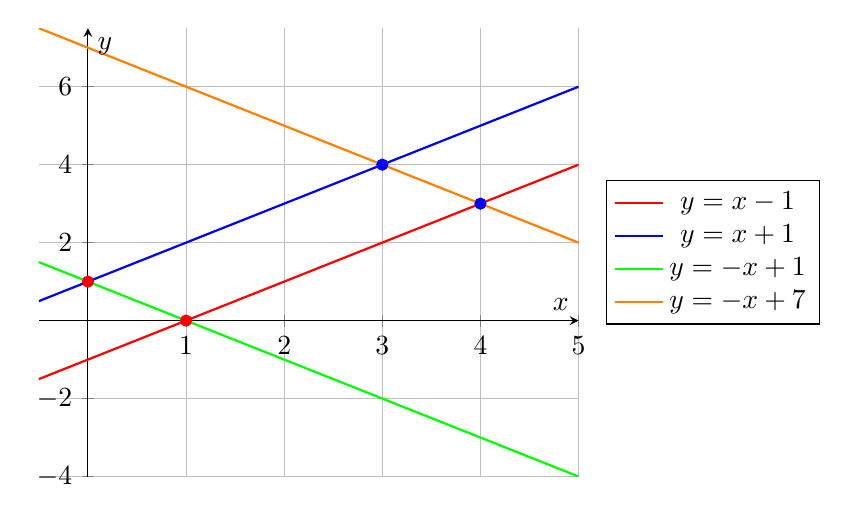
\begin{tikzpicture}
        \begin{axis}[
            axis lines = middle,
            xlabel = {$x$},
            ylabel = {$y$},
            grid = major,
            domain = -0.5:5,
            legend style = {at={(1.05,0.5)}, anchor=west}
        ]
        \addplot[red, thick] {x - 1};
        \addlegendentry{$y = x - 1$}
    
        \addplot[blue, thick] {x + 1};
        \addlegendentry{$y = x + 1$}
    
        \addplot[green, thick] {-x + 1};
        \addlegendentry{$y = -x + 1$}
    
        \addplot[orange, thick] {-x + 7};
        \addlegendentry{$y = -x + 7$}

        \addplot[only marks, red] coordinates {(0,1) (1,0)};
        
        \addplot[only marks, blue] coordinates {(3,4) (4,3)};
        
        \end{axis}
    \end{tikzpicture}
    \end{center}

    Obteniendo las funciones que intersecan en los puntos $(0,1),(1,0),(3,4),(4,3)$, podemos realizar el cambio de variable:
    \begin{align}
        y &= x - 1 \\
        y &= x + 1 \\
        y &= -x + 1 \\
        y &= -x + 7
    \end{align}

    Despejando ecuaciones semejantes:
    \[
        u = y - x, \quad v = y + x.
    \]    
    Donde 
    \[
        -1\leq u \leq 1, \quad 1 \leq v \leq 7.
    \]

    \subsection*{Transformación de variables}
    Sumando y restando las dos ecuaciones se despeja $x$ y $y$
    \[
        x = \frac{u + v}{2}, \quad y = \frac{v - u}{2}.
    \]

    \vspace{10pt}
    Por lo que llegamos a $T(u,v) = (\frac{u + v}{2},\frac{u - v}{2})$

    \subsection*{Determinante Jacobiano}
    \[
    \frac{\partial(x, y)}{\partial(u, v)}  =  \begin{vmatrix} 
        \frac{1}{2} & \frac{1}{2} \\ \\ 
        -\frac{1}{2} & \frac{1}{2} 
    \end{vmatrix} = \frac{1}{4} - \left(-\frac{1}{4}\right) = \frac{1}{2}
    \]

    Con esto:
    \begin{align*}
        \iint_B (x+y) \, dx \, dy &= \int \limits_{1}^{7} \int \limits_{-1}^{1} \frac{1}{2}\left(\frac{v - u}{2} + \frac{v + u}{2} \right) \, du \, dv \\
        &=\frac{1}{2} \int \limits_{1}^{7} \int \limits_{-1}^{1} v \, du \, dv \\
        &= \frac{1}{2}\int \limits_{1}^{7} 2v \,dv \\
        &= \frac{v^2}{2} \Big|^{7}_{1} \\
        &= \frac{49}{1} - \frac{1}{2} \\
        &= 24
    \end{align*}
